\chapter{Project Plan \& Project Phase Description}

\section{Long-term Plan}

The initial long-term plan can be seen in Figure \ref*{fig:longTermPlan}.

\begin{figure}[!ht]
    \centering
    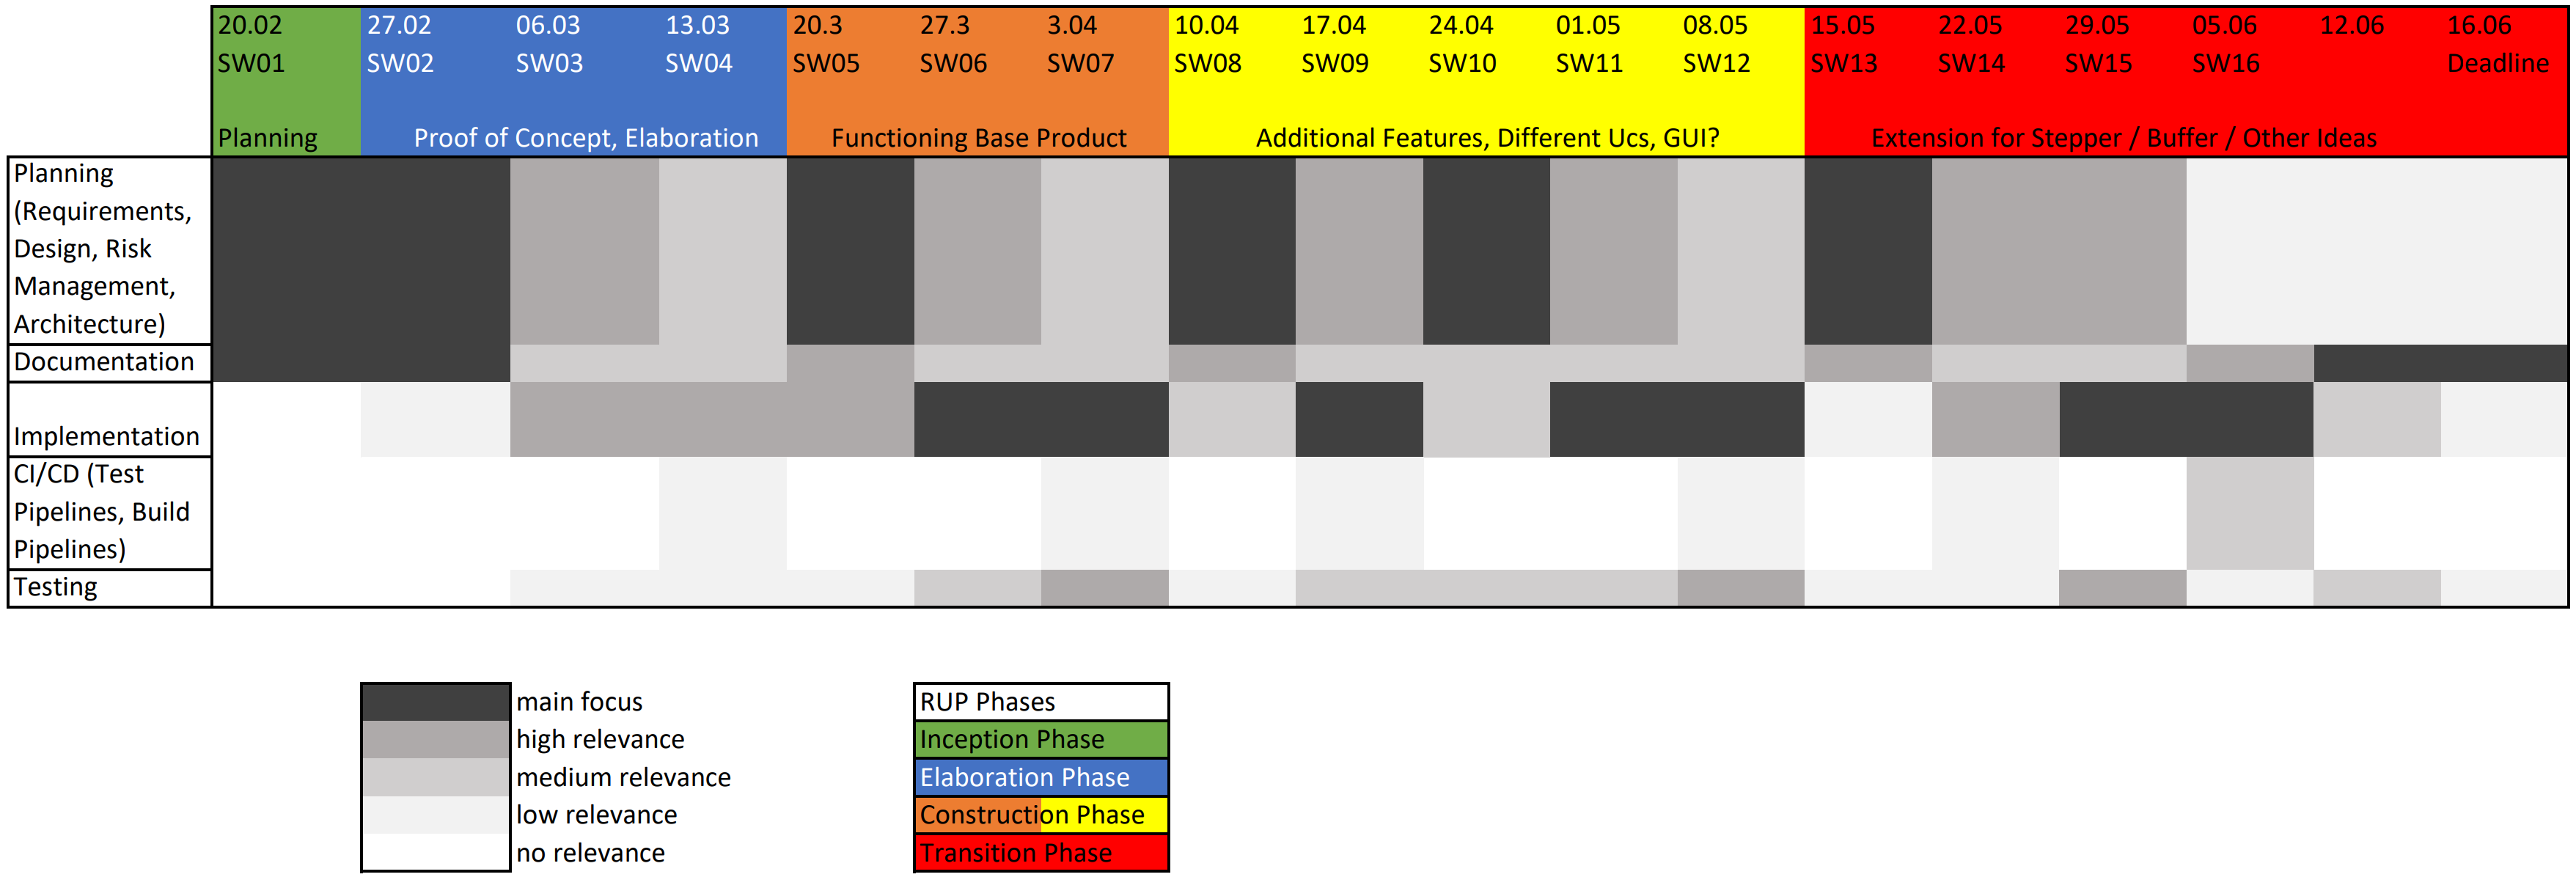
\includegraphics[width=0.96\textheight,angle=270]{resources/LongTermPlan.PNG}
    \caption{Initial Long-Term Project Plan, created around end of February}
    \label{fig:longTermPlan}
\end{figure}

Over the course of the project,
the long-term plan had to be adjusted multiple times because of a slightly changing scope and certain tasks taking longer than initially estimated.

Around the middle of March, the project was lagging behind the original plan already.
It took longer than expected to get familiar with Core and to fully understand what is going on.

In addition, I was working on a suitable data structure for the derivation of the terms.
While at the start I tried some more complex things,
like a tree of trees to be able to contain every possible step at once,
this turned out to be too complex and not really necessary.
So in the end I settled on the \texttt{Derivation} data structure,
that only supports the current history of \texttt{DerivationSteps}.
Another thing that I worked on was the \texttt{Term}/\texttt{Subterm} data structure.
Finding a suitable data structure that did not have to make use of the Maybe monad was a bit complicated,
and in the end,
I decided to go with the solution that Mr. Mehta suggested.

After figuring out that maybe sharing was not very desirable in the Substitution Stepper as it complicates certain things,
I also started working on an alternative stepper to the CoreStepper that did not include the sharing and thus simplified the stepping and displaying of the term.

For these reasons,
the initial elaboration phase took longer than expected,
as can be seen in \ref*{fig:longTermPlanMarch}.
The elaboration phase was prolonged by a week.
Since there was still a buffer at the end of the project,
this could be done easily.

\begin{figure}[!ht]
    \centering
    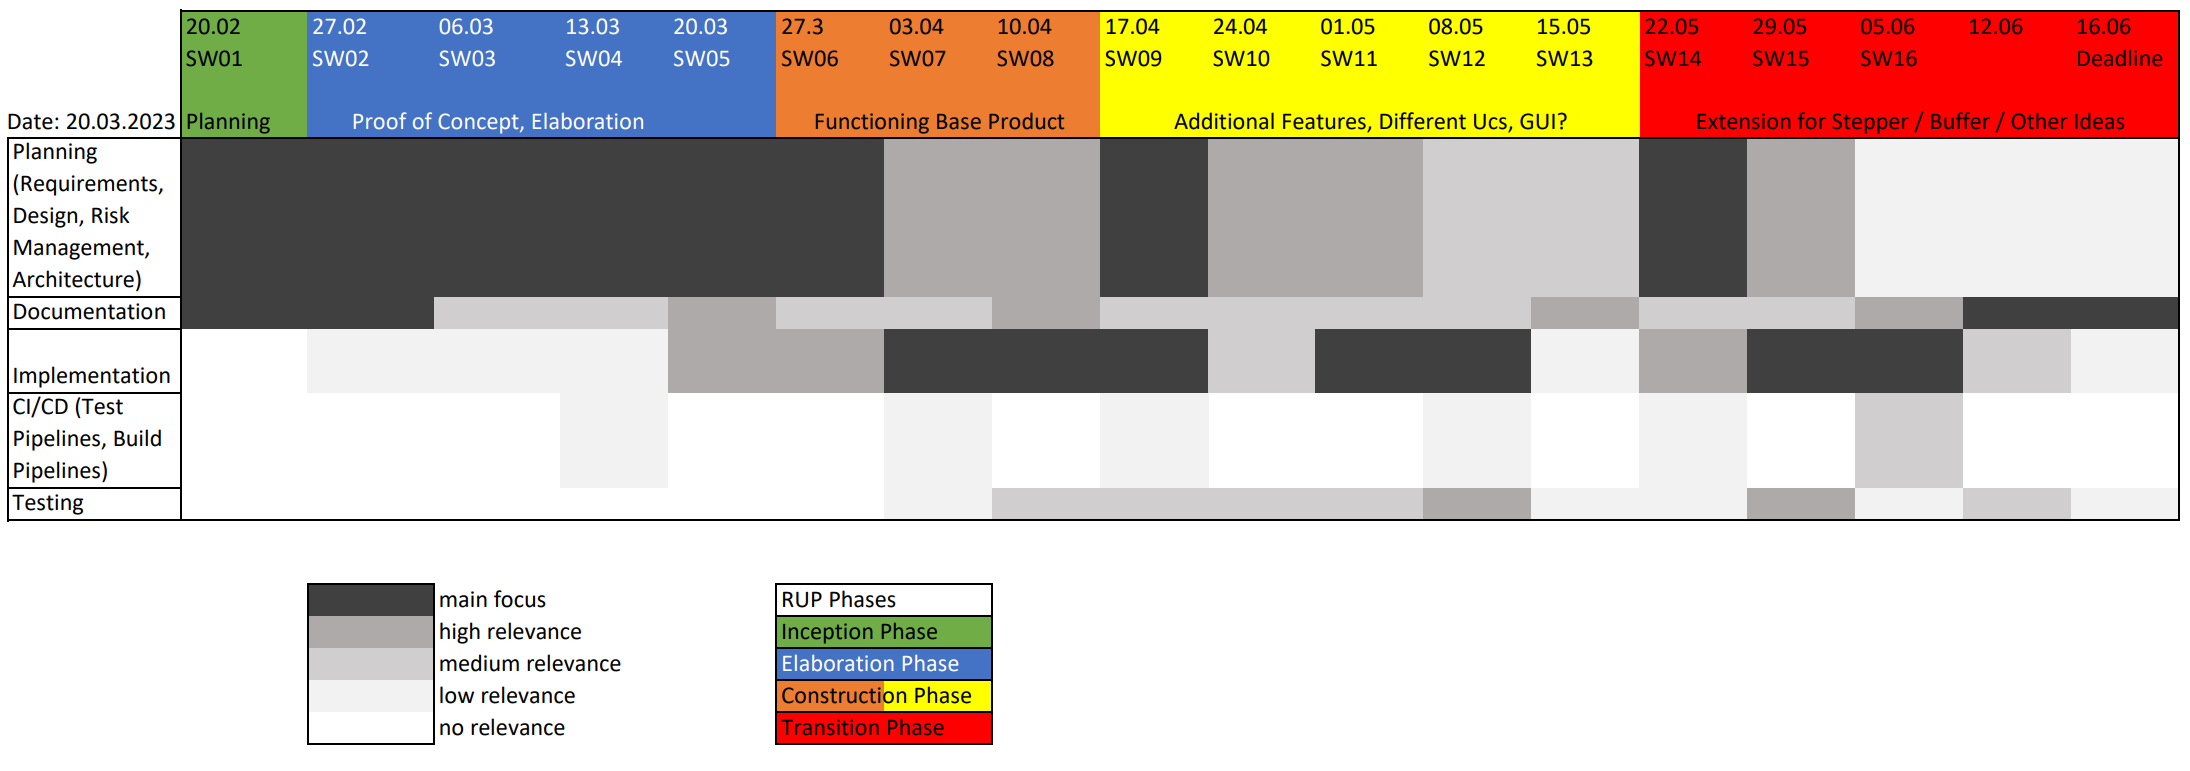
\includegraphics[width=0.96\textheight,angle=270]{resources/LongTermPlanMarch.PNG}
    \caption{Second version of the long-term plan created after the elaboration phase.}
    \label{fig:longTermPlanMarch}
\end{figure}

The second time the long-term plan was re-evaluated was in the middle of April.
The prototype of the Substitution stepper was working.
The user was able to select which subterm to step next and the terms were looking presentable.
However, this took also longer than expected.
Because of the re-implementation of the stepping which took a while to get right.

The changes made during that time can be seen in \ref*{fig:longTermPlanApril}.
The first part of the construction phase was prolonged by a week,
and again the time was subtracted from the buffer.

\begin{figure}[!ht]
    \centering
    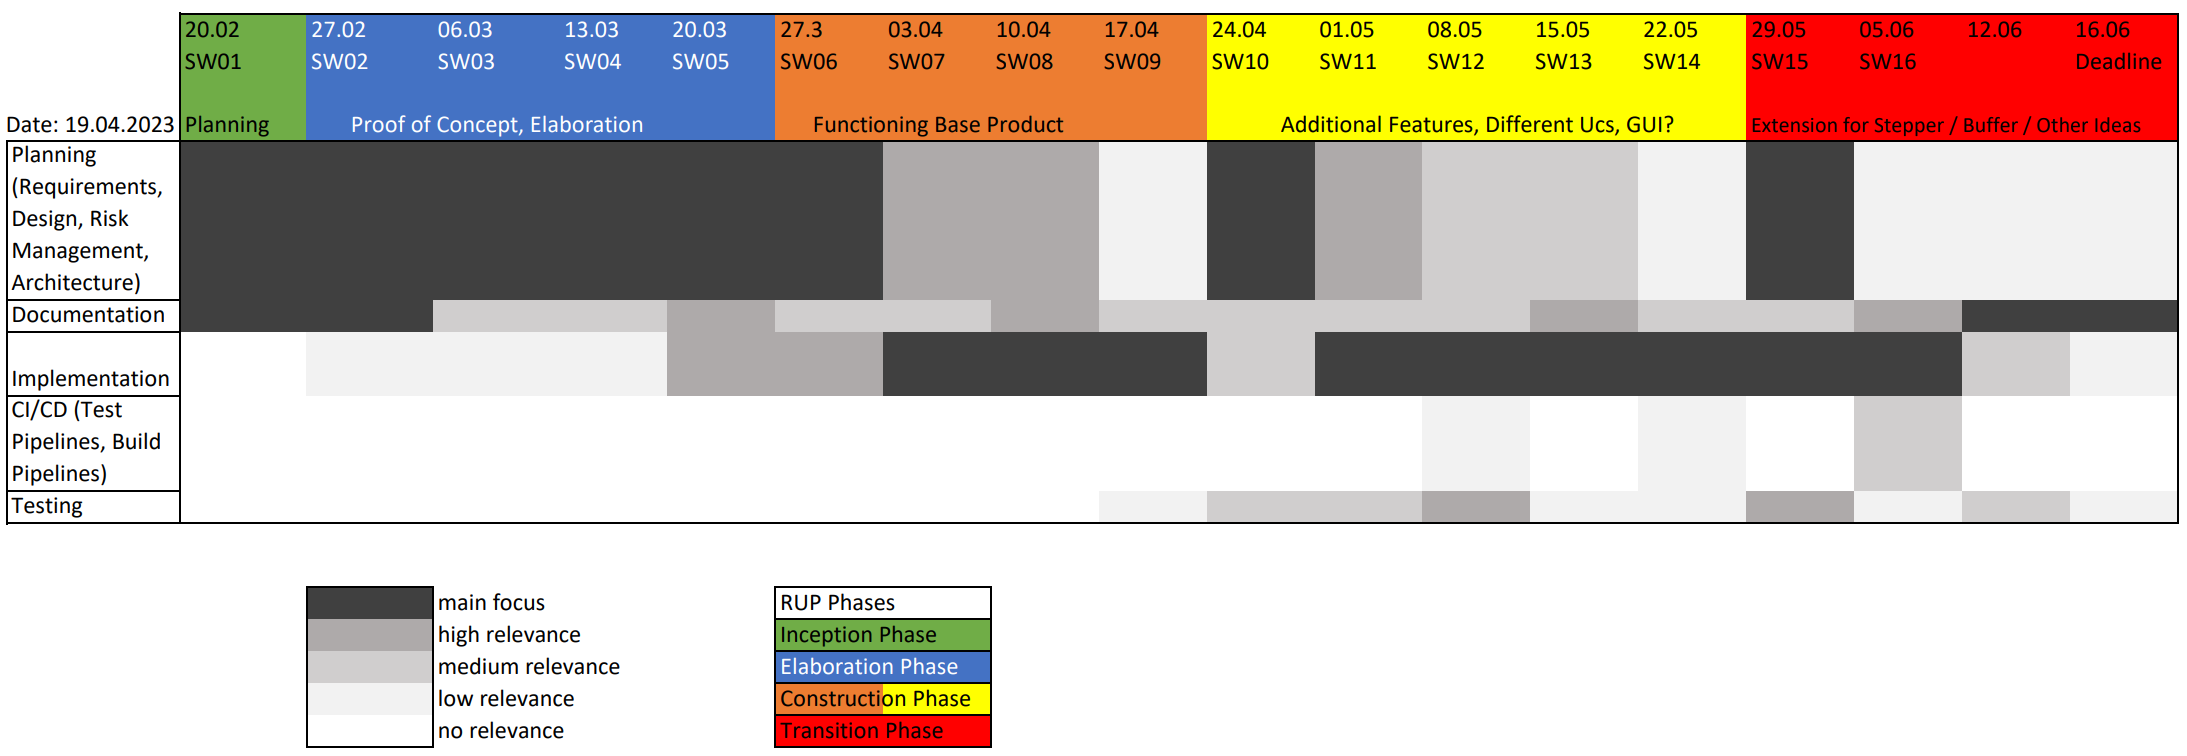
\includegraphics[width=0.96\textheight,angle=270]{resources/LongTermPlanApril.PNG}
    \caption{Second version of the long-term plan created after the prototype was working.}
    \label{fig:longTermPlanApril}
\end{figure}

The last time the long-term plan was adjusted was in the middle of May.
The prototype had been extended with multiple features that improve quality of life and make the Substitution Stepper more usable.
All of these features were part of the initially created requirements.
The second part of the construction phase took longer than expected as well,
further reducing the time that was planned as a buffer.
Because of that, there was no time for another requirement analysis and subsequent extension of the Substitution Stepper towards the end of the project.
The last two to three weeks of the project were reserved for the documentation.

Unfortunately,
due to the tightness of the schedule and the fact that most things took longer than expected,
certain things like testing needed to be cut from the plan, which is also indicated in the different iterations of the plan.

The final plan can be seen in \ref*{fig:longTermPlanMay}

\begin{figure}[!ht]
    \centering
    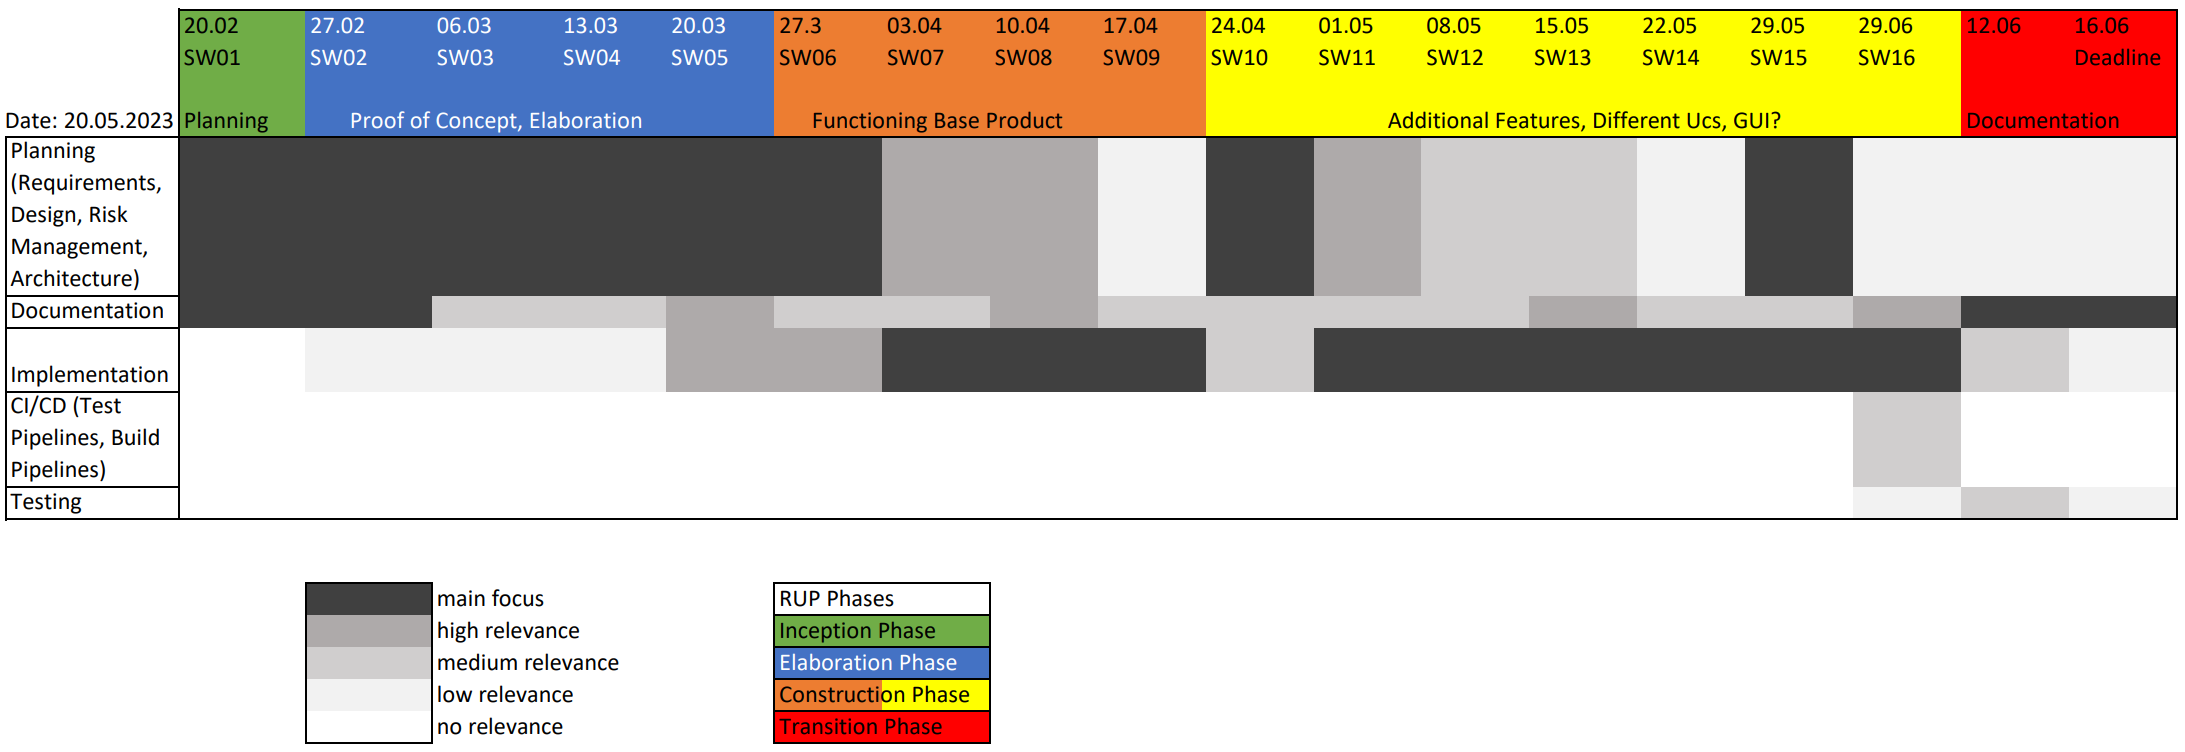
\includegraphics[width=0.96\textheight,angle=270]{resources/LongTermPlanMay.PNG}
    \caption{Last version of the long-term plan created.}
    \label{fig:longTermPlanMay}
\end{figure}

